\documentclass[4:3]{lecture}
\usepackage{amsmath,amssymb,inconsolata,relsize,bm,xcolor,hyperref,multicol,booktabs,suffix,overpic}
\usepackage[fixed]{fontawesome5} 

% Colors
\definecolor{backgroundlightgray}{gray}{0.97}
\colorlet{hidden}{mediumgray}
\definecolor{fsublue}{RGB}{0,47,93}

% Macros
\newcommand{\query}[1]{\textbf{{\texttt{\smaller #1}}}\xspace}

\let\item\itemaux
\newcommand{\faItem}[1]{\item[\smaller\faIcon{#1}\hspace*{-0.4em}]}
\WithSuffix\newcommand\faItem*[1]{\item[\smaller\smaller\raisebox{0.1ex}{\faIcon{#1}}\hspace*{-0.4em}]}

\newcommand{\paperTitle}{Axiomatic IR... but for RAG?!}
\bsauthor{Heinrich}
\bsyear{2025}

\begin{document}

\pagestyle{empty}

\begin{bsslide}
  \begin{center}
    \hfill\vfill 
    {\large Axiomatic IR... but for Retrieval-Augmented Generation?!}
    {\color{fsublue}\rule{\textwidth}{1.5pt}}
    \vspace*{0.25ex}
    Heinrich
    \begin{center}
      
\includegraphics[width=0.7\linewidth]{meme-distracted}\\[-1.5ex]
    \end{center}
    \vfill
  \end{center}
\end{bsslide}

\begin{bsslide}[\paperTitle]
  \vspace*{1ex}
  \colortext{\faIcon{flag-checkered} Traditional goal: Constraints between pairs of \textbf{retrieved documents}}
  \vspace*{1.5ex}\\
  \begin{minipage}{0.25\linewidth}
    
\includegraphics[width=\linewidth]{meme-boring}    
  \end{minipage}
  {\Large\faIcon{caret-right}}
  \begin{minipage}{0.6\linewidth}
    \fbox{
      \begin{overpic}[width=\linewidth]{screenshot-ir-axioms}
        \put(80,12){
\includegraphics[width=0.3\linewidth]{stamp-completed}}
        \put(15,5){\rotatebox{-5}{\colorbox{white}{\fbox{\Large TFC1}}}}
        \put(35,8){\rotatebox{-2}{\colorbox{white}{\fbox{\Large LNC1}}}}
        \put(50,2){\rotatebox{10}{\colorbox{white}{\fbox{\Large STMC2}}}}
        \put(5,9){\rotatebox{8}{\colorbox{white}{\fbox{\Large PROX4}}}}
      \end{overpic}
    }
  \end{minipage}
\end{bsslide}
\begin{bsslide}[\paperTitle]
  \lastslide
  \vspace*{2.5ex}\\
  \begin{minipage}{0.50\linewidth}
    
\includegraphics[width=\linewidth]{meme-everywhere}      
  \end{minipage}
  {\Large\faIcon{caret-right}}
  \hspace*{-1em}\begin{minipage}{0.37\linewidth}
    \begin{itemize}
      \item \sout{SERP} {\footnotesize\faIcon{arrow-right}} answer
      \item \sout{result} {\footnotesize\faIcon{arrow-right}} context\\[-0.5ex]
      \Large\color{\altcolor}
      \item \sout{search} {\normalsize\faIcon{arrow-right}} \textbf{RAG}\\
      \footnotesize (Retrieval-Augmented Generation)
    \end{itemize}
  \end{minipage}
\end{bsslide}

\newcommand{\comparisonImage}{figure-comparison-axes}
\begin{bsslide}[\paperTitle]
  \vspace*{1ex}
  \sout{\textcolor{gray}{\faIcon[regular]{flag} Traditional goal: Constraints between pairs of retrieved documents}}

  \vspace*{1ex}
  \colortext{\faIcon{flag-checkered} Goal: Constraints between pairs of \textbf{generated answers}}
  \vspace*{2ex}
  \begin{center}
    \includegraphics[width=0.9\linewidth]{\comparisonImage}      
  \end{center}
\end{bsslide}
\renewcommand{\comparisonImage}{meme-one-does-not}
\begin{bsslide}[\paperTitle]
  \lastslide
\end{bsslide}

\begin{bsslide}[\paperTitle]
  \vspace*{1ex}
  \colortext{\faIcon{exchange-alt} New axioms for RAG}

  \begin{center}
    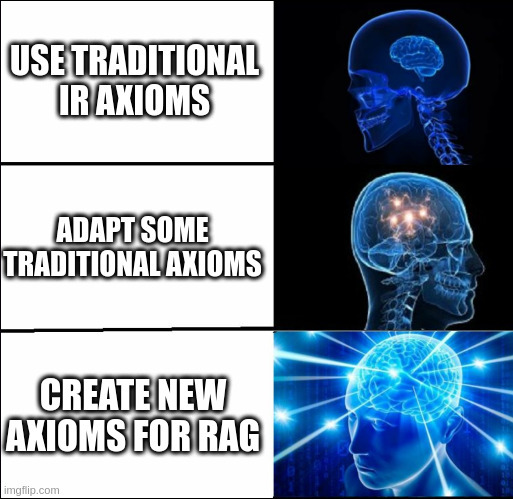
\includegraphics[width=0.64\linewidth]{meme-galaxy-brain}      
  \end{center}
\end{bsslide}

\begin{bsslide}[\paperTitle]
  \vspace*{1ex}
  \colortext{\faIcon{exchange-alt} New axioms for RAG}
  \vspace{2ex}

  \begin{minipage}[c]{0.26\linewidth}
    \textbf{Criteria} \bscite{Lukas\,@\,SIGIR'24}\kern-0.5em
    \begin{itemize}
      \setlength{\itemsep}{0.5ex}
      \setlength{\itemindent}{-1em}
      \faItem{pencil-alt} Coherence
      \faItem{expand-arrows-alt} Coverage
      \faItem{folder-open} Consistency
      \faItem{shield-alt} Correctness
      \faItem{universal-access} Clarity
    \end{itemize}
  \end{minipage}%
  {\Large\faIcon{caret-right}}%
  \begin{minipage}[c]{0.36\linewidth}
    \textbf{Axioms} 
    \begin{itemize}
      \setlength{\itemsep}{0.5ex}
      \setlength{\itemindent}{-1em}
      \item COH1,\,COH2
      \item COV1,\,COV2,\,COV3
      \item CONS1,\,CONS2,\,CONS3
      \item CORR1
      \item CLAR1,\,CLAR2
    \end{itemize}
  \end{minipage}%
  {\Large\faIcon{caret-right}}%
  \begin{minipage}[c]{0.27\linewidth}
    \textbf{Experiments}
    \begin{itemize}
      \setlength{\itemsep}{0.5ex}
      \setlength{\itemindent}{-1em}
      \item TREC RAG'24
      \item human prefs.\bscite{Lukas}
      \item 3 LLMs
      \faItem{arrow-right} axiom consistency
      \faItem{arrow-right} ax.\ decisiveness
    \end{itemize}
  \end{minipage}\\[3.5ex]
  \begin{center}
    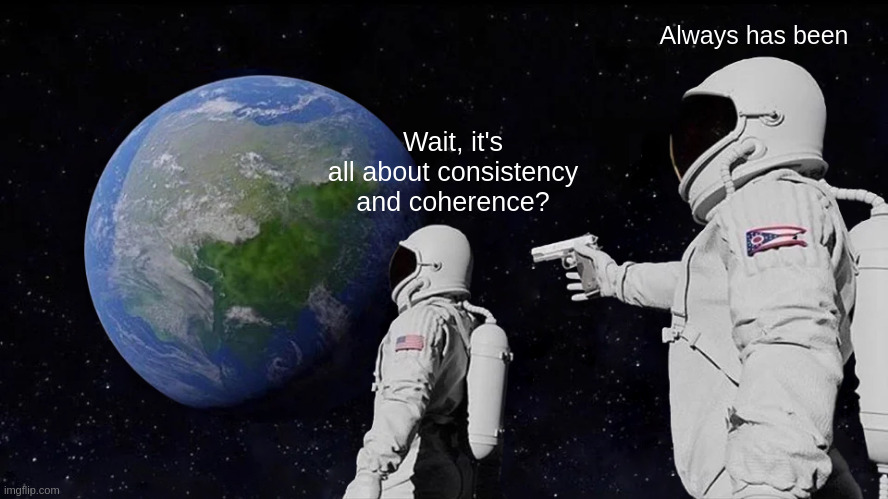
\includegraphics[width=0.57\linewidth]{meme-all-about}    
  \end{center}
\end{bsslide}

\colorlet{colorA}{white}
\begin{bsslide}[\paperTitle]
  \vspace*{1ex}
  \colortext{Results}\\[1ex]
  \begin{minipage}{0.40\linewidth}
    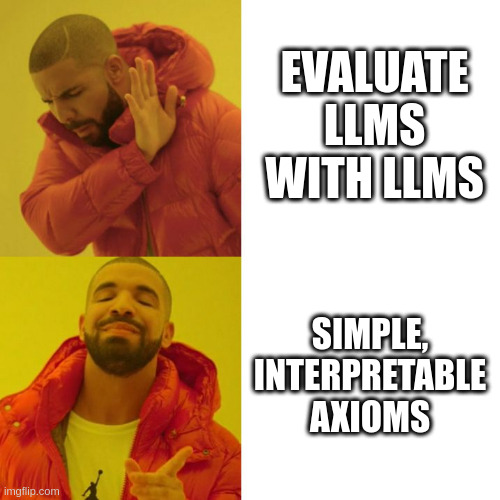
\includegraphics[width=\linewidth]{meme-nah}\\[2ex]
    
\includegraphics[width=\linewidth]{meme-my-part}
  \end{minipage}
  \hfill
  \begin{minipage}{0.34\linewidth}
    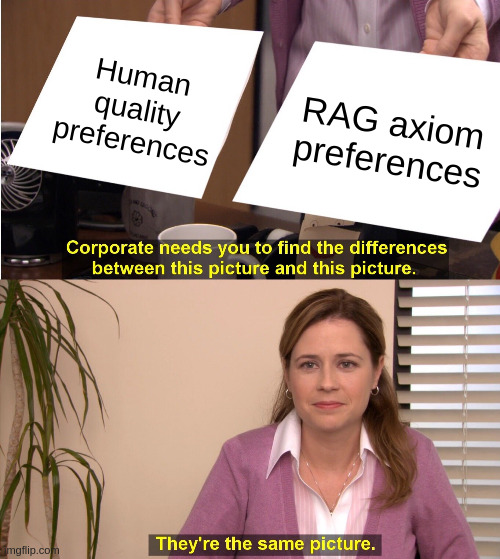
\includegraphics[width=\linewidth]{meme-corporate}\\[2ex]
    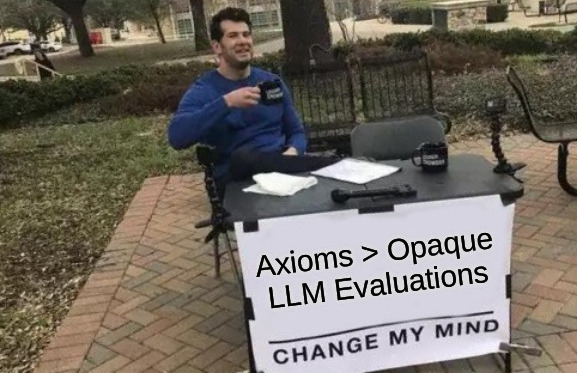
\includegraphics[width=\linewidth]{meme-change}
  \end{minipage}
  \hfill
  \begin{minipage}{0.2\linewidth}
    TL;DR \faIcon{itunes-note}\\
    {\footnotesize``The Axiom Anthem''}\\[1ex]
    
\includegraphics[width=\linewidth]{qr-code-song}\\[20ex]
    \begin{flushright}
      \textcolor{colorA}{\large\emph{Thank you!}}
    \end{flushright}
  \end{minipage}\\
\end{bsslide}
\colorlet{colorA}{black}
\begin{bsslide}[\paperTitle]
    \lastslide
\end{bsslide}

\end{document}
